% Autor: Martin Hofbauer, Brno 2022
% ###########################################################################
\chapter{Úvod}
% ###########################################################################
TODO

\chapter{Výběr technologií}

TODO

\section{Programovací jazyk}

Jednou z nejdůležitějších částí při výběru použitých technologií je právě programovací jazyk. V našem případě je nutné zvolit takový, ve kterém aplikace poběží velmi rychle. Také je důležité volit jazyk kompilovaný, aby na cílových zařízeních nemusel být přítomný interpret (kvůli zpomalenému vykonávání kódu a také rychlosti nasazování aplikace bez nutnosti instalovat dodatečné programy). Po zvážení všech vyjmenovaných požadavků jsme si vybrali programovací jazyk C++. Mohl by se také použít programovací jazyk C, ale C++ nabízí objektové programování a v kombinaci se systémem CMake je možné vytvářet hezky čitelný kód s jednoduchou správou knihoven třetích stran.




\section{Meziprocesní komunikace}
TODO(k čemu)
\subsection{Roury}
\subsection{TCP/IP}
TODO(co jsem vybral)



% ###########################################################################
\chapter{Návrh systému}
% ###########################################################################

Aplikaci chceme mít rozdělenou do dvou konceptuálních celků - agenti, kteří se budou starat o samostatné sbírání informací ze systému a jádrem, kterému budou tyto informace zasílány a následně je bude zpracovávat. Důležité je, aby selhání agenta neovlivnilo zbytek aplikace, takže jako nejlepší řešení se nabízí, že agenti budou samostatně běžící procesy, které svým selháním nemůžou ukončit celou aplikaci. 

Rozdělíme tedy systém do tří částí: Core, Communication, AgentClient.
\section*{Core}
Tato část bude jádrem celého programu. Na začátku vykonávání se postará o přečtení požadovaných agentů. Následně tyto agenty postupně začne jako samostatné procesy pouštět, během toho s nimi naváže spojení, vymění si s nimi potřebné informace a následně začne přijímat zaznamenané informace. Pokud během vytváření alespoň u jednoho agenta nastane chyba a nenaváže se spojení nebo něco podobného, tak je celý program ukončen. 

Jádro poté přijímá zasílané informace agentů do té doby, dokud program není přerušen signálem nebo dokud nejsou všichni agenti ukončeni. V případě přerušení musí všechny agenty ukončit a následně ukončit i sebe.

Na obrázku \ref{systemArchitecture} vidíme.

\begin{figure}[hbt]
	\centering
	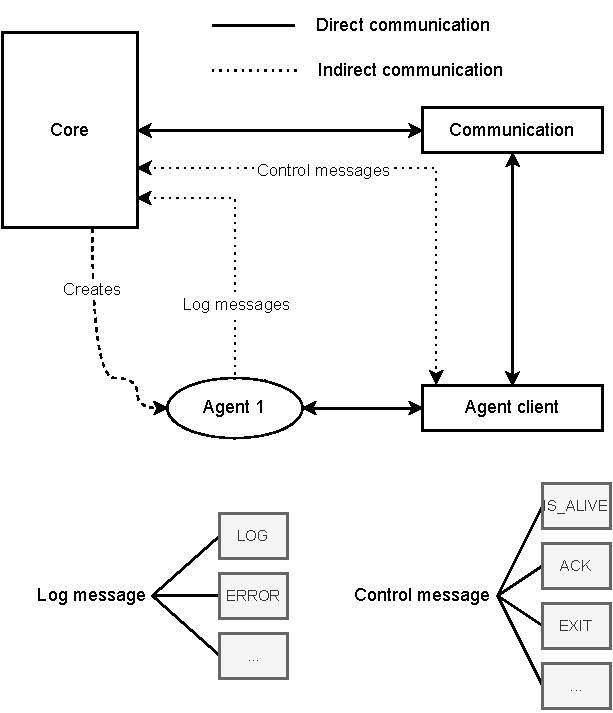
\includegraphics[width=\textwidth]{diagrams/architecture/architecture_diagram.pdf}
	\caption{Architektura systému}
    \label{systemArchitecture}
\end{figure}

% ###########################################################################
\chapter{Implementace}
% ###########################################################################
\begin{figure}[hbt]
	\centering
	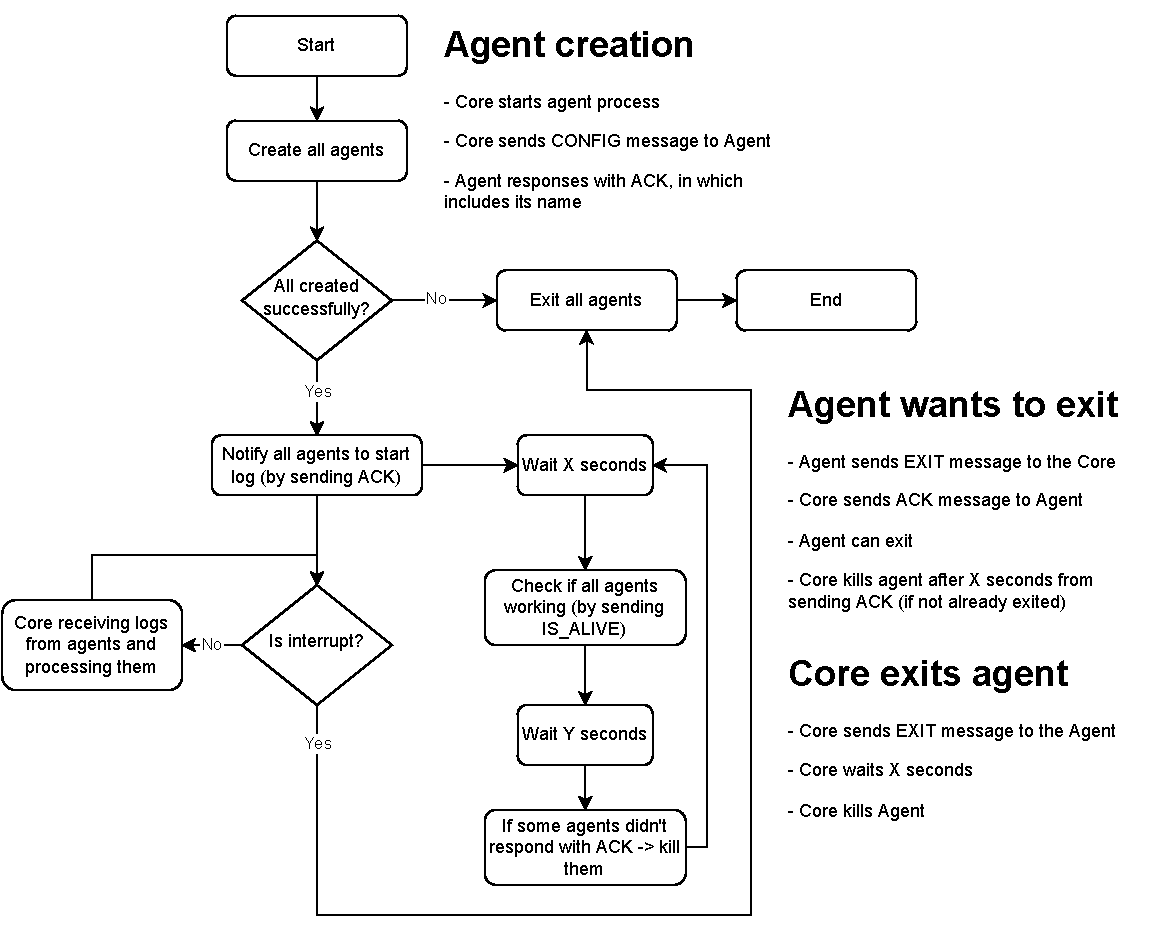
\includegraphics[width=\textwidth]{diagrams/flowchart/flowchart.pdf}
	\caption{Vývojový diagram chování systému}
\end{figure}
\begin{figure}[hbt]
	\centering
	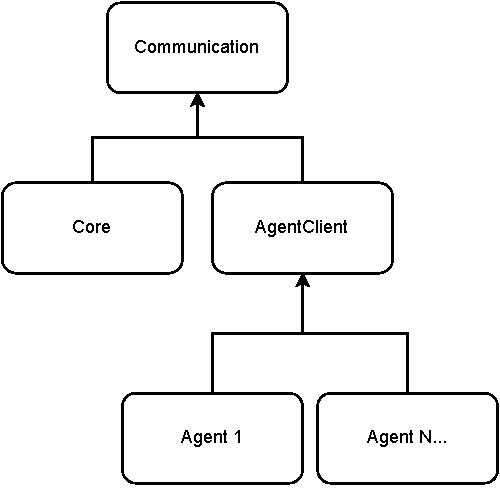
\includegraphics[width=\textwidth]{diagrams/dependency-diagram/dependency_diagram.pdf}
	\caption{Diagram závislostí}
\end{figure}

% ###########################################################################
\chapter{Testování}
% ###########################################################################
TODO

% ###########################################################################
\chapter{Závěr}
% ###########################################################################
TODO



